\documentclass[12px]{article}

\usepackage{babel}
\usepackage[T1]{fontenc}
\usepackage[a4paper]{geometry}
\usepackage{hyperref}
\usepackage[utf8]{inputenc}
\usepackage{mathtools}
\usepackage{pdfpages}
\usepackage[textsize=small]{todonotes}
\usepackage{xcolor}


\title{%
  Internship Report --- M2 MPRI \\
  Constant delay enumeration for documents spanners
}
\author{Rémi Dupré}


\begin{document}
  \maketitle

  \subsection*{The general context}

  % What is it about ?
  % Where does it come from ?
  % What is the state of the art in this area ?

  % NOTE: citations concernant les méthodes classiques ?
  The problem of membership for regular languages is a well-understood problem,
  automata-based techniques. \pierre{The previous sentence is
  nonsensical}  
  % NOTE: illisible
  However, few efforts have been made to enumerate all matches of a regexp over
  a text. Indeed most tools used to match regexps only produce one match, some
  like grep are intended to find any line containing a match, it sometimes
  append \pierre{happen} that an option is available to list all
  non-overlapping matches. \pierre{Previous sentence likes coordination
  (conjunctions, etc.)}
  % "the tools intended to list all matches only list non-overlapping..."

  Enumeration techniques are widely used in database theory, \pierre{Not
  sure it is useful to mention database theory here} in order to deal
  with large datasets, it seems relevant to try applying these techniques for
  the problem of enumerating matches over a text, which could result on a
  quadratic output for large input documents. \pierre{The sentence is too
  long and it is not clear what the message is}
  % dire y a bcp then dire c'est pour ca algo enumeration

\subsection*{The research problem}

  % What is the question that you studied ?
  % Why is it important, what are the applications/consequences ?
  % Is it a new problem ?
  % If so, why are you the first researcher in the universe who consider it ?
  % If not, why did you think that you could bring an original contribution ?

  My internship focuses on an algorithm proposed by Antoine Amarilli, Pierre
  Bourhis, Stefan Mengel and Matthias Niewerth~\cite{ICDT19}, it allows to
  enumerate all matches of a regexp with a constant delay, and a preprocessing
  linear in the size of the automata \pierre{automaton, not automata; but
  is it in the size of the automaton, or in that of the document?}
  \pierre{Break the sentence in two or use conjunctions to structure the
  sentence}
  (complexity factors dependent of the
  size of the regular expression being considered as constants).
  \pierre{This is not understandable: how does the size of the regular
  expression and the size of the automaton differs?}
  % need a def of constant

  No implementation was provided for this algorithm yet, and it seemed that
  some new issues would appear while trying to implement the algorithm, for
  example the memory cost of a naive implementation of the algorithm would
  quickly exceed the typical memory available on a personal computer.
  % semms like no pb, "in particular investigating new questions [...]"

\subsection*{Your contribution}

  % What is your solution to the question described in the last paragraph ?
  % Be careful, do \emph{not} give technical details, only rough ideas !
  % Pay a special attention to the description  of the \emph{scientific}
  % approach.

\subsection*{Arguments supporting its validity}

  % What is the evidence that your solution is a good solution ?  Experiments ?
  % Proofs ?
  % Comment the robustness of your solution: how does it rely/depend on the
  % working assumptions ?

\subsection*{Summary and future work}

  % What is next ? In which respect is your approach general ?
  % What did your contribution bring to the area ?
  % What should be done now ?
  % What is the good \emph{next} question ?

  \pagebreak


  \section{Introduction}

    The problem of finding a substring from a text belonging to a given
    regular language has been widely studied. In particular Thompson
    introduced an automata based approach in
    1968~\cite{thompson1968programming} which is now known as one of the
    fastest implementation for regular expressions~\cite{cox2007regular}.

    However, as classical approaches simulate runs over a regular automaton
    while reading the input document linearly, they cannot output two
    substrings that overlap each over. Take the examples of the regexp
    \texttt{\textcolor{blue}{AUG}\textcolor{gray}{(.\{3\})\{0,2\}}\textcolor{red}{UAA}},
    matching any substring in the form $uvw \in \Sigma^*$ where $u =
    \text{\textcolor{blue}{AUG}}$, $|v| \in \{0, 3, 6\}$ and $w =
    \text{\textcolor{red}{UAA}}$. It has 3 matches over the document $d =
    \texttt{AUGAUGTGTUAAUAA}$:
    \begin{itemize}
      \item $d_0 \ldots d_8 =
        \texttt{\textcolor{blue}{AUG}\textcolor{gray}{AUGTGT}\textcolor{red}{UAA}}$
      \item $d_3 \ldots d_8 =
        \texttt{\textcolor{blue}{AUG}\textcolor{gray}{TGT}\textcolor{red}{UAA}}$
      \item $d_3 \ldots d_{11} =
        \texttt{\textcolor{blue}{AUG}\textcolor{gray}{TGTUAA}\textcolor{red}{UAA}}$
    \end{itemize}

    By allowing overlapping matches, it also mean that the can could be of
    a quadratic size in the size of the input document. Thus, a classical
    worst case complexity analysis cannot hope to be faster than $O(|d|^2)$.
    This worst case behaviour is fairly easy to reach using the regex
    \texttt{.*} over any document $d$.

    Since the input of a pattern matching problem is typically big, this
    quadratic factor is usually too expensive. Moreover, in many real world
    cases, the output will actually be very small compared to the input.

    Thus it will be more relevant to use a different complexity measure for
    this problem, which is expressive about the size of the output. Here, we
    will use the complexity of enumeration, which integrates two measures:

    \begin{itemize}
      \item an upper bound on the time spent in the \textit{preprocessing}
        phase of the algorithm, this is the time spent computing before the
        first result is outputted.
      \item an upper bound on the \textit{delay} of the algorithm, this is
        the maximum time elapsed between the output of two results of the
        algorithm.
    \end{itemize}

    Amarilli~\&~al.~\cite{ICDT19} introduced an enumeration algorithm with a
    preprocessing phase linear in the size of the input document, and a delay
    independent of this size. My work was to adapt this algorithm for
    implementation and compare it to other existing tools.


  \section{Definitions}

    \subsection{Regular expressions and regular languages}

      \subsubsection{Regular expressions}

        The language of regular expressions over an alphabet $\Sigma$ can
        recursively be defined as the language containing:

        \begin{itemize}
          \item $``\emptyset"$ denoting the empty set of words of $\Sigma$
          \item $``\epsilon"$ denoting the set containing only the empty string
          \item $\forall a \in \Sigma, ``a"$ denoting the set
            containing only the character a
          \item for any regular expressions $E_1$ and $E_2$, $``E_1 E_2"$
            denoting the set of concatenations of a word of $E_1$ with a word
            of $E_2$.
          \item for any regular expressions $E_1$ and $E_2$, $E_1|E_2$
            denoting the union of words of $E_1$ and $E_2$.
          \item for any regular expression $E$, $E^*$ denoting the set
            containing $epsilon$ and any other concatenation of words of $E$.
        \end{itemize}

        The languages denoted by regular expressions are regular languages,
        they are also the languages recognised by finite automata.

        \paragraph{Notations} Some extra syntax can be introduced to make the
        regular expressions more pleasant to use, some of it will be used to
        make examples more readable in this report:
        \begin{itemize}
          \item $``."$ denotes the entire alphabet $\Sigma$
          \item for any regular expression $E$ and $0 \leq n \leq m$,
            $``E\{n,m\}"$ denotes the languages of words containing
            concatenation of between $n$ and $m$ words of $E$. $``E\{n\}"$
            denotes the set of words that are concatenation of exactly $n$
            words of $E$.
          \item closure has an higher precedence than concatenation which has
            higher precedence than union: \texttt{hello|world!*} denotes the
            set $\{hello, world, world!, world!!, world!!!, \ldots\}$
        \end{itemize}

      \subsubsection{Classical algorithms}

        Given a deterministic finite automaton $\mathcal{A}$, naively running
        the automaton a document $d$ takes time $O(|d|)$ and determines whether
        $d$ is part of the language recognised by $\mathcal{A}$.

        If $\mathcal{A}$ is not deterministic, it is still possible to perform
        the same operation in time $O(|\mathcal{A}| |d|)$: it requires to
        simulate all possible runs by keeping the set $Q_i$ of all possible
        states of the execution of $A$ while reading $d_i$. If $\mathcal{A} =
        (Q, I, \delta, F)$:
        \begin{itemize}
          \item $Q_0 = I$
          \item $\forall 1 \leq i \leq |d|, Q_i = \{(q', d_i, q'') \in \delta,
            q' \in Q_{i-1}\}$
        \end{itemize}
        Finally, there is a valid run of $\mathcal{A}$ over $d$ if $Q_{|d|}
        \bigcap F \neq \emptyset$.

        \vspace{0.5cm}

        The next main issue is then to find an automata that recognises the
        language of an input regular expression. Thompson algorithm introduces
        operation to recursively apply the operations of union, concatenation
        and closure to the automatons representing
        subexpressions~\cite{thompson1968programming}. This process is linear
        in the size of the expression but the resulting automata is not
        minimal unless the $\epsilon$-transitions are removed, which can take a
        time in $O(n^2)$.

        Glushkov algorithm in the other hand can also compute a minimal
        automata, by recursively computing the set of the first letters, last
        letters and factor two of the words in the regular
        language~\cite{glushkov1961abstract}\todo{check the source}. This
        process takes time $O(n^2)$.

    \subsection{Variable set automata}

      \subsubsection*{Document spanner}

        Let $\Sigma$ be a finite alphabet. A document $d = d_0 \dots d_{n-1}$
        is a word over $\Sigma$. A \textit{span} of $d$ is a pair $[i,
        j\rangle$ with $0 \leq i \leq j \leq |d|$ which represents a substring
        of $d$ starting at position $i$ and ending at position $j - 1$.

        Given a finite set $\mathcal{V}$ of variables, a result is defined as a
        \textit{mapping} from these variables to spans of the input document.
        Note that some variable may remain unassigned: formally, a mapping of
        $\mathcal{V}$ on $d$ is a function $\mu$ from some domain
        $\mathcal{V}_0 \subset \mathcal{V}$ to spans of $d$.

        We define a \textit{document spanner} to be a function assigning to
        every input document d a set of mappings, which denotes the set of
        results of the extraction task on the document d.

      \subsubsection*{Sequential Variable Set Automata}

        Document spanners will here be represented using \textit{variable-set}
        automata (VAs). The transition of a VA can either hold a letter of
        $\Sigma$ or a \textit{variable marker} $x \vdash$ (denoting the
        start of a span assigning to $x$), or $\dashv x$ (denoting the end of
        a span assigning to $x$), where $x \in \mathcal{V}$.

        Similarly to a classical automaton, a VA is defined as a tuple $A = (Q,
        q_0, F, \delta)$ where $\delta$ defines a set of \textit{transitions}
        of the form $(q, \sigma, q')$ where $\sigma \in \Sigma$ for
        \textit{letter transitions} or $\sigma \in \mathcal{V}$ for
        \textit{variable transitions}.

        A run $\sigma$ of $A$ over $d$ is defined as a sequence of
        configurations
          \[ (q_0, i_0) \xrightarrow{\sigma_1} (q_1, i_1)
          \xrightarrow{\sigma_2} \ldots \xrightarrow{\sigma_m} (q_m, i_m) \]
        where $i_0 = 0$, $i_m = |d|$ and for every $1 \leq j \leq m$:
        \begin{itemize}
          \item Either $\sigma_j$ is a letter of $\Sigma$, we have $i_j =
            i_{j-1} + 1$, $d_{i_{j-1}} = \sigma_j$ and $(q_{j-1}, \sigma_j,
            q_j)$ is a letter transition of $A$;
          \item Or $\sigma_j$ is a variable marker, we have $i_j = i_{j-1}$,
            and $(q_{j-1}, \sigma_j, q_j)$ is a variable transition of $A$. In
            this case we say that the variable marker $\sigma_j$ is read at
            position $i_j$.
        \end{itemize}

        A run is \textit{valid} if it is accepting ($q_m \in F$), every
        variable marker is read at most once, and whenever an open marker $x
        \vdash$ is read at a position $i$ then the corresponding close marker
        $\dashv x$ is read at a position $i'$ with $i \leq i'$ .

        The algorithm will only take as input automata that can't be accepting
        but not valid. Such an automaton is called \textit{sequential}. Note
        that it is NP-complete to decide if a VA has a valid run over a
        document~\cite{freydenberger:LIPIcs:2017}. Also note that the problem
        of deciding if an automaton is sequential is in NL and that an
        automaton can be transformed into a sequential automaton with an
        exponential blowup.

        From each valid run a mapping is defined where each variable $x \in V$
        is mapped to the span $[i, i'\rangle$ such that $x \dashv$ is read at
        position $i$ and $\vdash x$ is read at position $i'$ ; if these markers
        are not read then $x$ is not assigned by the mapping (i.e., it is not
        in the domain $\mathcal{V}_0$). The document spanner of the VA $A$ is
        then the function that assigns to every document $d$ the set of
        mappings defined by the valid runs of $A$ on $d$: note that the same
        mapping can be defined by multiple different runs.

        The task of the enumeration algorithm defined in~\cite{ICDT19} is the
        following: given a VA $A$ and a document $d$, enumerate without
        duplicates the mappings that are assigned to $d$ by the document
        spanner of $A$.

    \subsection{Example(s)}
      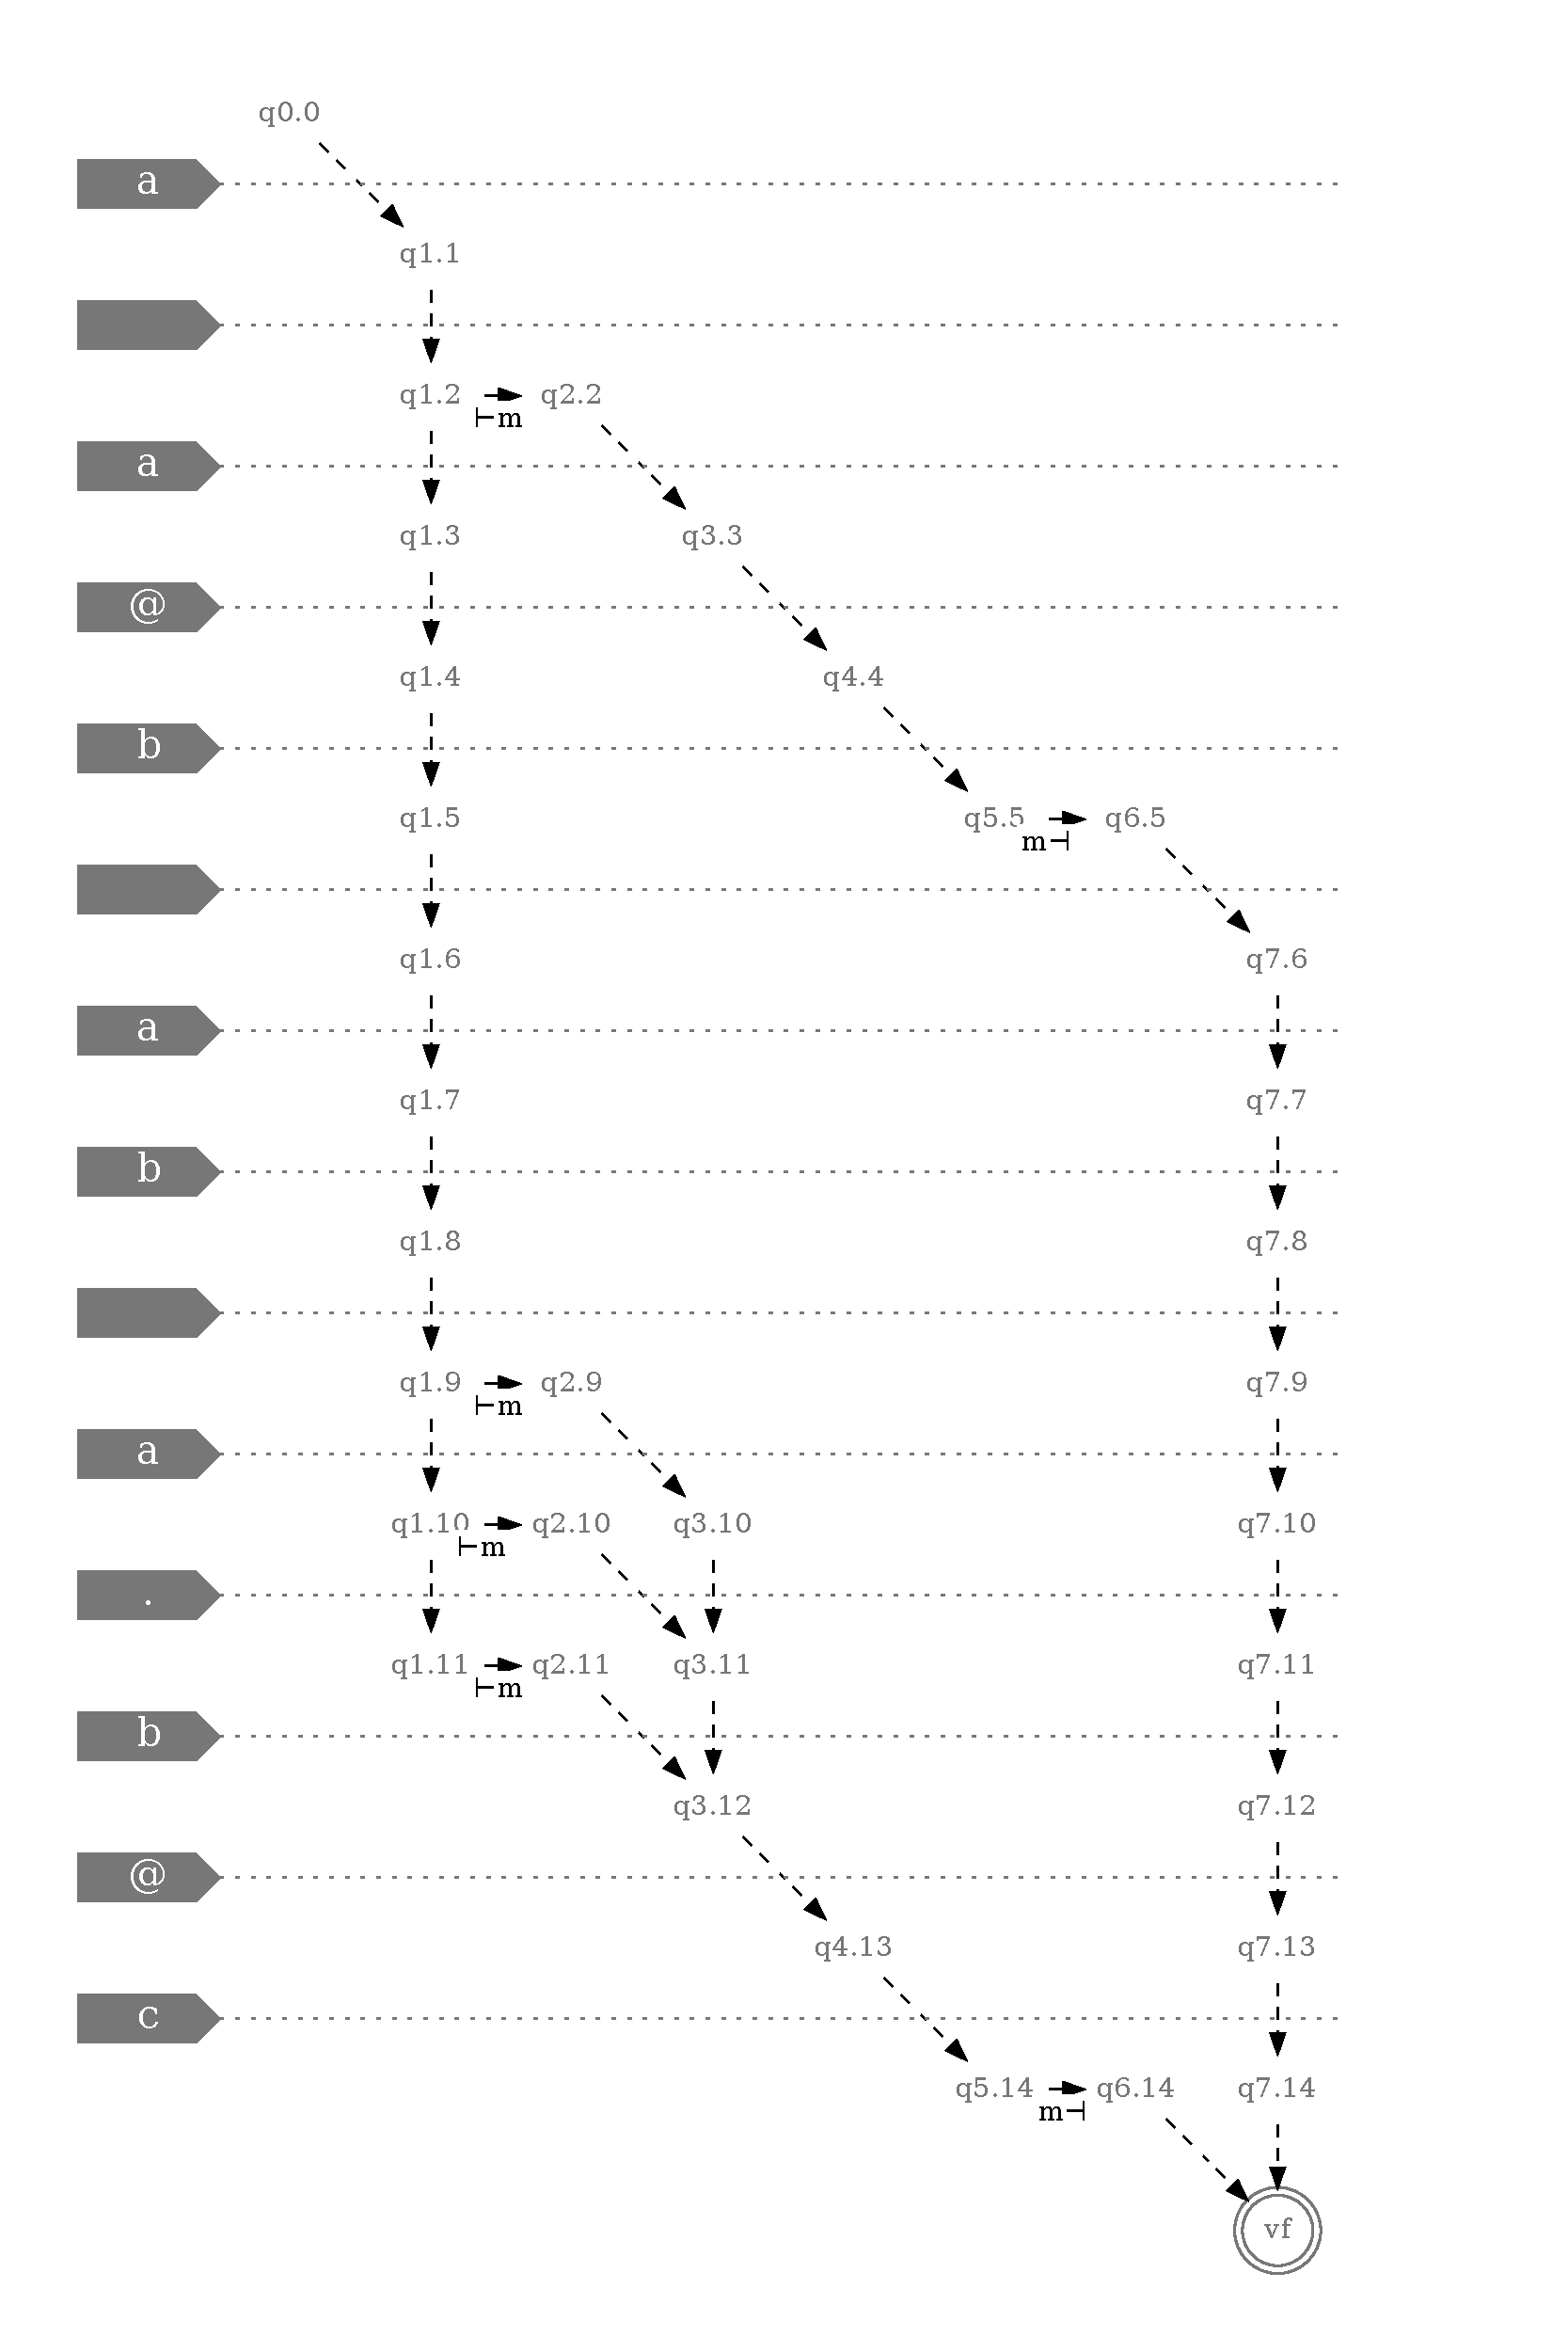
\includepdf{figures/example_dag.pdf}

    \subsection{Related work}

      % - Christiano & al
      % - anything else ?


  \section{Outline of the enumeration algorithm}


  \section{Implementation}

    % Some implementation details, out of a subsection

    \subsection{Technical details}

      A first draft of the implementation of the algorithm was implemented
      using Python 3, this programming language is known to be slow but its
      flexibility allowed to get a working implementation after about a week of
      work. The expression are parsed using a LALR parser for a custom grammar,
      and are converted to an automata using the Glushkov algorithm.

      I later built an implementation using Rust in order to be able to compare
      performances of the algorithm with existing tools without suffering of
      the overhead of Python. The regex crate of Rust allows to access the
      AST of parsed regexps, but I still needed to compile the into automaton
      using Glushkov algorithm in order to handle variables.

      These tools work similarly to other pattern matching tools like grep and
      use the same regex syntax. Variables are defined out of named groups, and
      instead of outputting a single match with a single assignation to groups,
      it outputs the list of all possible assignations of groups of the
      expressions.

      \todo{Introduire le naïf quelque-part par ici?}.

    \subsection{Limitations}

      \todo[inline]{trucs pas time efficient (hashtables, matrices?)}

    \subsection{Cleaning unreachable states}


  \section{Performance of the algorithm}

    \subsection{Limitations of existing tools}

      Excepted for the naive algorithms and the work of Florenzano \&
      al.~\todo{reference}, it is difficult to fairly compare to already
      existing tools. Some of these tools allow to output a list of overlapping
      matches, however this will at most output one match for each starting
      position in the output document. Regex actually have a greedy semantic
      for closures in the context of these tools, it will as a default match
      the largest possible string for each closure and can be turned to a lazy
      semantic where it only matches the smallest possible string. For
      example,\todo{todo}.

    \subsection{Results}


  \pagebreak
  \bibliography{bibliography}
  \bibliographystyle{ieeetr}

\end{document}
